\documentclass[../main.tex]{subfiles}
\begin{document}

\section{Experimentelle Validierung}

\subsection{Datenerfassung}
Ziel ist ein Verfahren zu entwickeln, das ein digitales Abbild von einem realen Objekt
erstellen kann.
Als Grundlage für dieses Abbild arbeite ich in diesem Fall mit Pointclouds, 
die mithilfe eines Laserscanners aufgenommen wurden. Auch andere Möglichkeiten
Pointclouds zu erhalten sind denkbar und sollten mit dem Verfahren 
kompatibel sein. In den folgenden Absatz werde ich das Erstellen von Pointclouds 
mithilfe eines Laserscanners erläutern und auf ein Verfahren eingehen, dass aus 
den Pointclouds digitale Objekte erstellt, die miteinander verglichen werden können.


\newpage

\begin{wrapfigure}{l}{0.25\textwidth}
    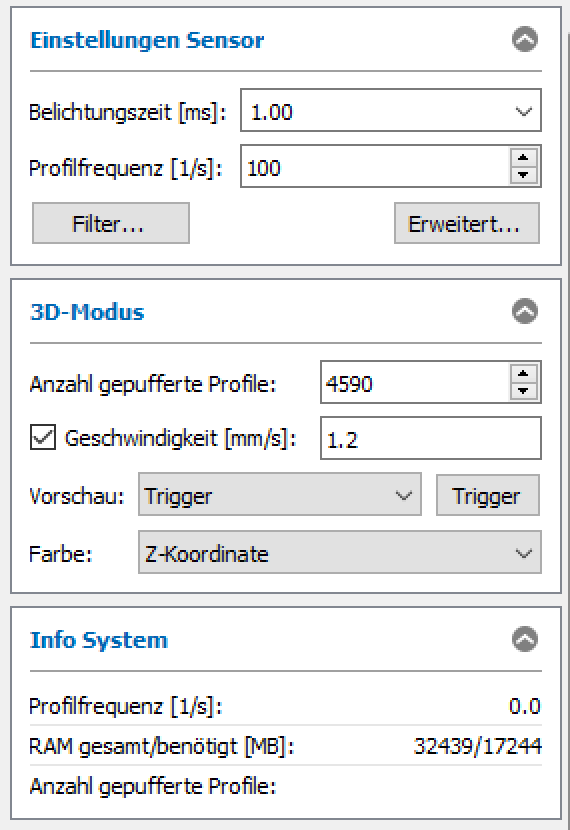
\includegraphics[width=0.25\textwidth]{images/Parameter_Scan.png}
    \caption{Scanparameter}
    \label{fig:scanparameter}
\end{wrapfigure}

\subsubsection{Limitierung der Achsen:}

Die gesamte Länge des Objekts kann also erfasst werden, indem Scanner 
beziehungsweise Werkzeugkopf in X-Richtung verschoben wird. Mit dem Start der 
Bewegung muss auch die Aufzeichnung der Scannerdaten beginnen. In unserem Fall wurde
die Datenerfassung manuell per Hand im richtigen Zeitpunkt über die Software 
'SCANControl' von micro-epsilon gestartet. 
Eine mögliche Verbesserung ist es, diesen Vorgang zu automatisieren, indem der 
Scanner automatisch mit dem Start der Bewegung getriggert wird und die Aufzeichnung
startet. Die Länge der Aufzeichnung wird auch über die Software eingestellt. 
In Abbildung \ref{fig:scanparameter} sind die korrekten Parameter für das 
Demonstratorbauteil zu sehen. Über den Parameter 'Anzahl gepufferte Profile' kann 
die Länge der Aufzeichnung eingestellt werden. Limitiert wird dieser Parameter 
durch den verfügbaren Speicher auf dem Zielsystem. Es sollte auch darauf geachtet 
werden das der Scanner mindestens genauso lange bewegt wird wie Aufzeichnung läuft, 
ist dies nicht der Fall entsteht eine Pointcloud die einmal größer als notwendig ist, 
und außerdem am Ende der x-Achse nur wiederholende Profile beinhalten. 
Die y-Achse der Pointcloud wird durch den eingesetzten Scanner limitiert. 


\subsubsection{Geschwindigkeit}
Der Parameter `Geschwindigkeit` in Abbildung \ref{fig:scanparameter} muss der realen Vorlaufgeschwindigkeit des Scanners
entsprechen um eine korrekte und akkurate Pointcloud zu erhalten. Ist die 
Messgeschwindigkeit kleiner als die Bewegung des Scanners werden Profile doppelt 
aufgenommen, ist sie zu hoch werden Profile übersprungen und das Bauteil wirkt in 
der resultierende Pointcloud in X-Richtung gestreckt.

\subsubsection{Endergebnis}

Ist dieser Prozess erfolgreich
erhält, man eine Pointcloud der Oberfläche des Objekts. 
In Abbildung \ref{fig:pointcloud_big} ist eine solche Pointcloud eines einzelnes
Scanverlaufs dargestellt. In Abbildung \ref{fig:pointcloud_small} ist eine Nahaufnahme 
des mittleren Teils derselben Pointcloud zu sehen.
Hier sind die einzelnen Punkte sichtbar und man kann erkennen wie die Oberfläche 
aus tausenden Punkten aufgebaut ist. Bei einem Messbereich von 25 mm und 2048 
Punkten pro Profil \cite{SCANNER} sind das mehr als 80 Punkte pro mm in einem
y-Achse-Profil.
Zusätzlich kann man im rechten oberen 
Bereich Ausreißer sehen, warum diese das Verfahren erschweren und 
wie man sie entfernen kann folgt in den kommenden Kapiteln. Außerdem werde ich auch
auf die Struktur von Pointcloud Dateien noch eingehen.

\begin{figure}[h!]
    \centering
    \begin{minipage}{0.45\textwidth}
        \centering
        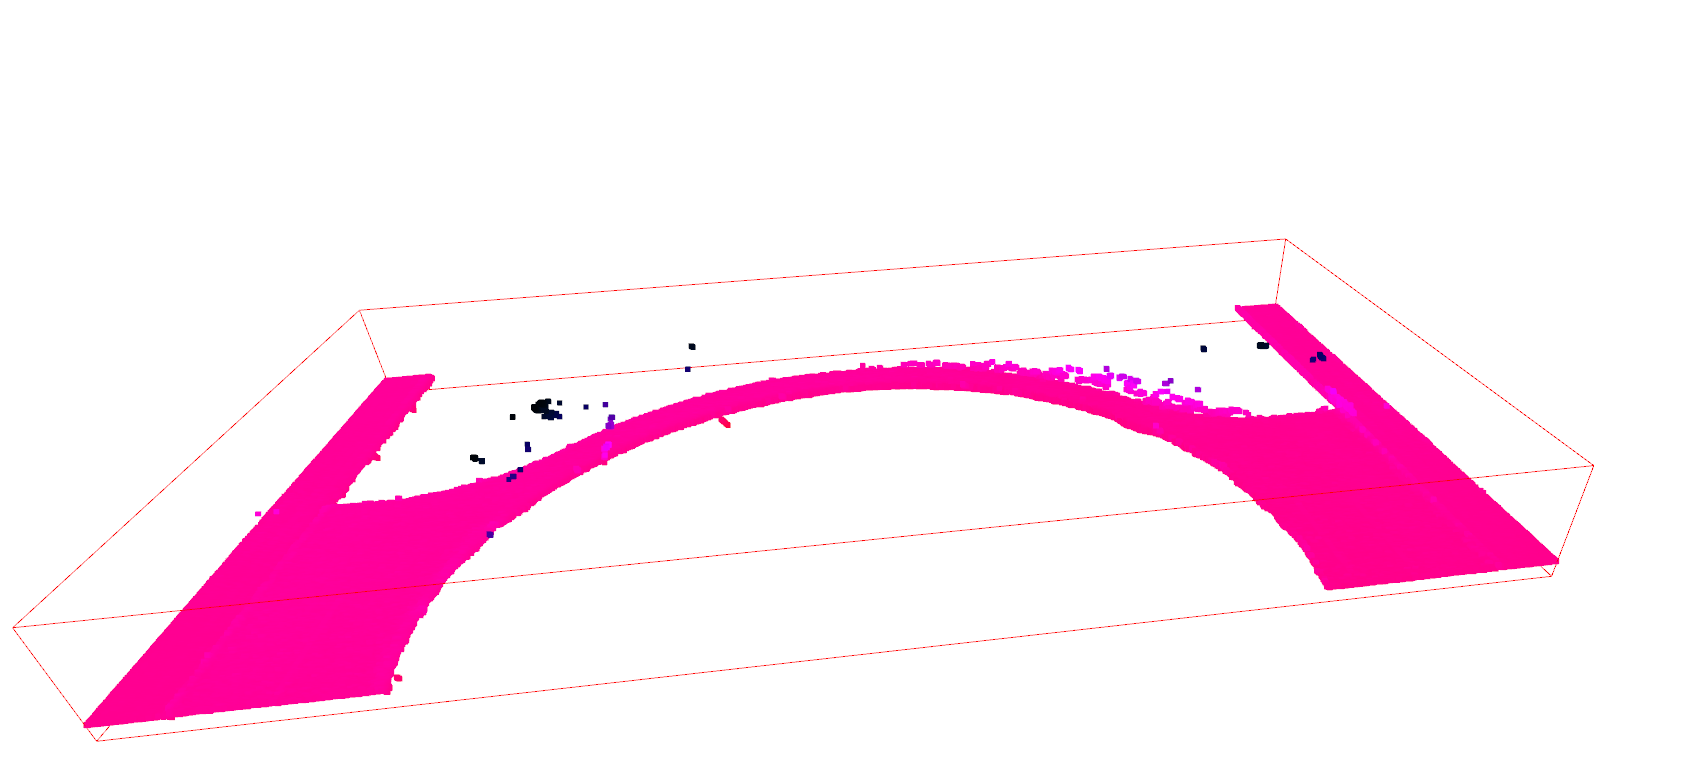
\includegraphics[width=0.9\textwidth]{images/pointcloud_big.PNG} % first figure itself
        \caption{Pointcloud}
        \label{fig:pointcloud_big}
    \end{minipage}\hfill
    \begin{minipage}{0.45\textwidth}
        \centering
        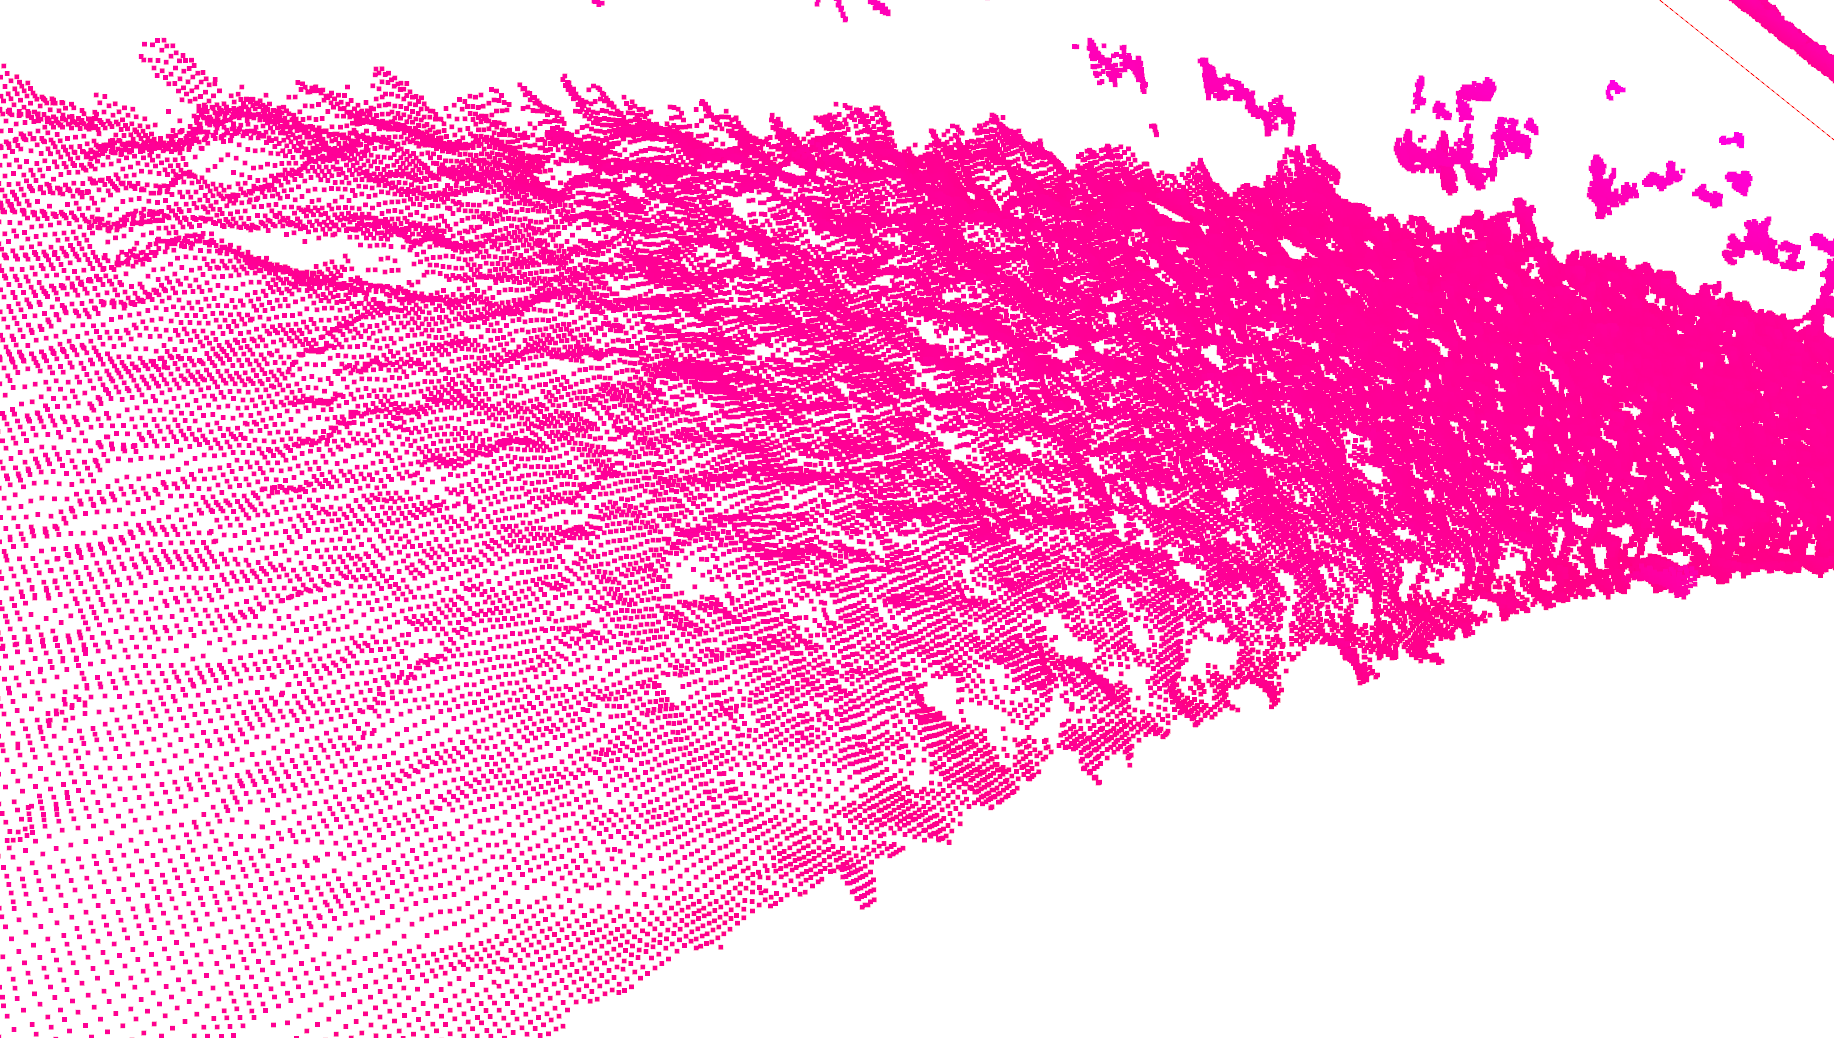
\includegraphics[width=0.9\textwidth]{images/pointcloud_small.PNG} % second figure itself
        \caption{Nahaufnahme Pointcloud}
        \label{fig:pointcloud_small}
    \end{minipage}
\end{figure}

\subsection*{Wahl des Demonstratorbauteils}

Man könnte sich jetzt hier die Frage stellen, warum das Demonstratorbauteil dann so gewählt 
und entworfen wurde das es symmetrisch ist. In dem ersten Schritt des zusammenfügen ist 
die Bauteilgeometrie zwar hinderlich, dafür profitiert die 
Spannkraftdeformationserkennung von dem initial runden Innenkreis des Bauteils.
Zusätzlich soll das hier zu entwickelnden Verfahren auf viele Bauteilgeometrien 
anwendbar sein und somit nicht durch eine Symmetrie beschränkt werden.

\subsection*{Weitere Verfahren}

Nachdem die globale Registrierung und der ICP-Algorithmus auf den Pointclouds nicht
anwendbar waren musste ein anderes Verfahren her. Aufgrund weniger schon existieren 
Verfahren die eine reine Bewegung auf nur 2 Achsen verwenden habe ich eine Idee 
entworfen, die auf dem ICP-Algorithmus basiert, um 2 Pointclouds zu vergleichen 
und zu verschieben. Hierfür habe ich die Pointclouds in ein zweidimensionales Array
mit den Z-Werten als Inhalt konvertiert. Nun kann die euklidische Distanz der Z-Werte
und jedem X und Y Wert aufsummiert werden. In einem naiven Ansatz kann dann eine 
Pointcloud entlang der Länge und Breite der anderen Pointcloud bewegt werden und für 
jede Transformation die Summe der Distanzen gespeichert werden. Die Idee war das die 
Transformation mit der kleinsten Summe die beste Überlappungen der beiden Pointclouds 
ist. Das hat aber nicht funktioniert. Durch die tatsächliche relativ kleine Überlappung 
ist die Summe der Distanzen nicht bei der korrekten Transformation minimal, 
sondern, wenn die Pointclouds maximal übereinander geschoben sind. Zusätzlich war die 
Verschiebung und Berechnung der zweidimensionalen Arrays rechenintensiv und hat zu 
langen Laufzeiten geführt. Also habe ich dieses Verfahren wieder aufgeben mit einer neuen
Idee:

\subsection{Pointcloud filtern}

\begin{wrapfigure}{r}{0.5\textwidth}
    \centering
    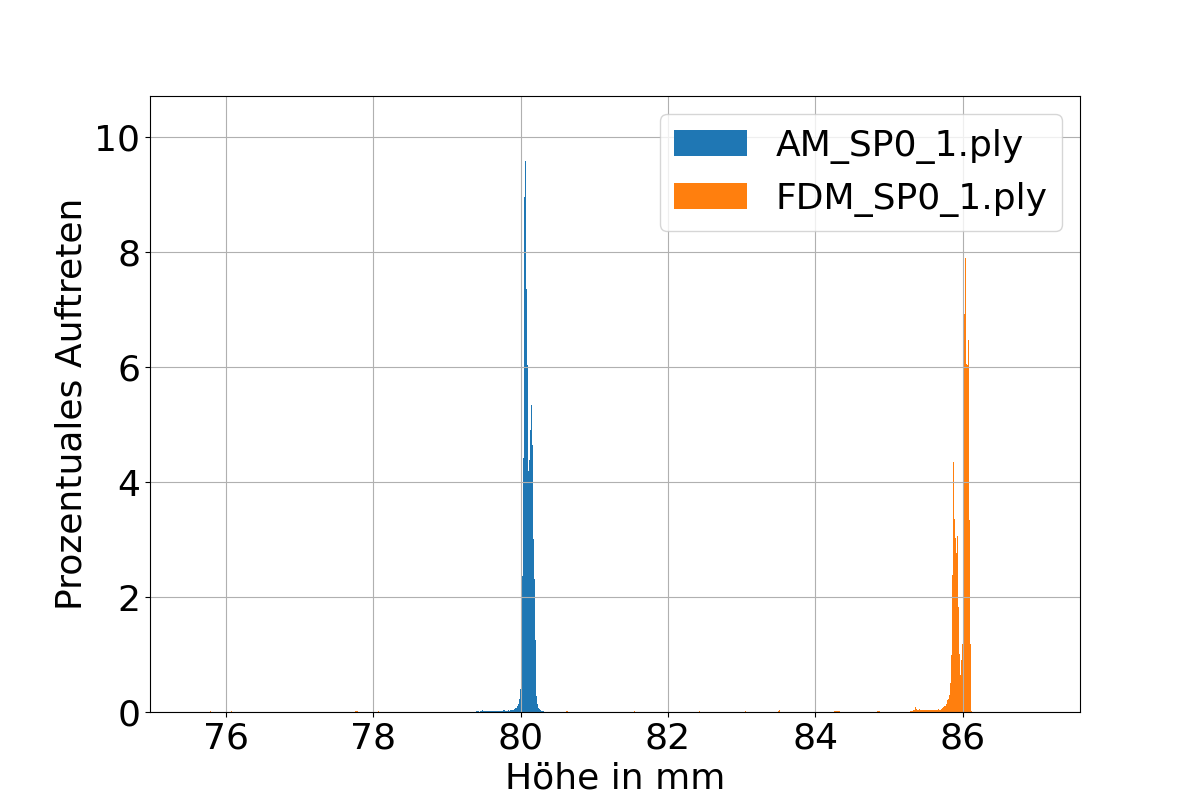
\includegraphics[width=0.5\textwidth]{images/height_occurange.png}
    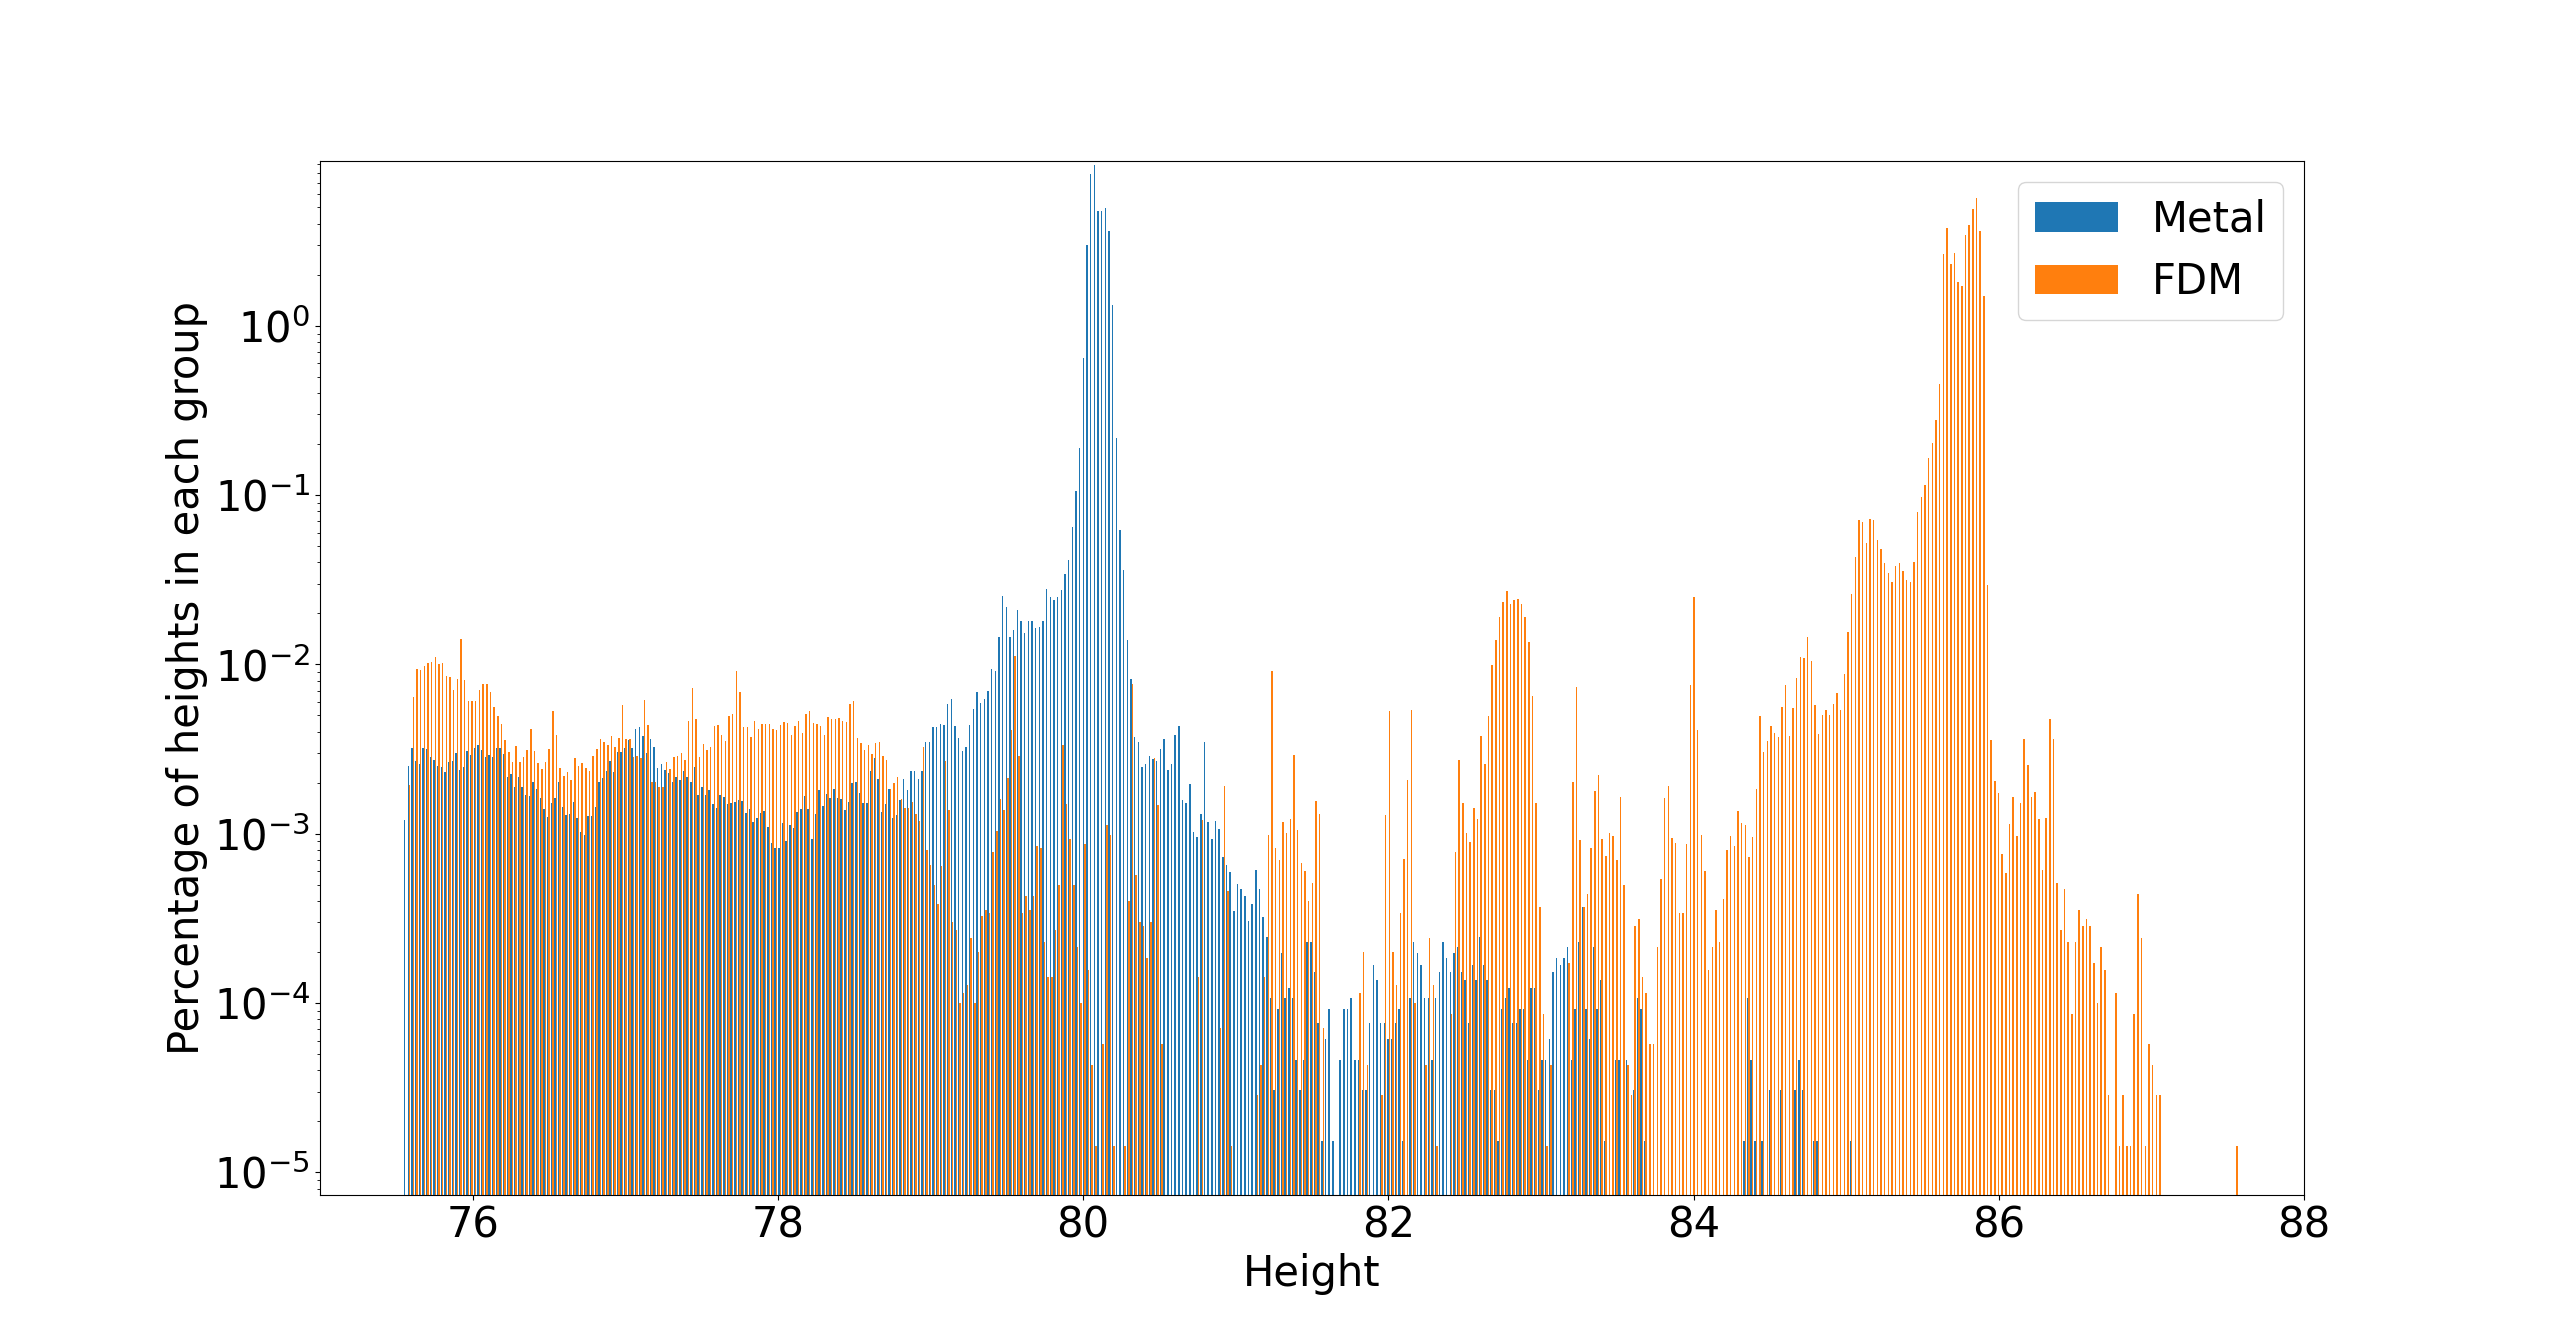
\includegraphics[width=0.5\textwidth]{images/height_occurange_log.png}
    \caption{Auftreten Höhe}
    \label{fig:brightness}
\end{wrapfigure}

Ziel ist ein Verfahren zu entwickelen Verfahren bei allen gängigen 
Additiven Fertigungsmethoden angewendet werden kann.
Das muss bei der Filterung der Daten berücksichtigt werden
da die Datenverteilung von FDM Bauteilen anders aussieht als bei Metallenen Werkstoffen, 
muss eine Pointcloud so gefiltert werden, dass das Zusammenfügen unabhängig von dem 
gewählten Material zuverlässig funktioniert.
Wie man in Abbildung \ref{fig:brightness} sehen kann streuen nicht alle Pointclouds 
gleich, abhängig von dem Werkstoff des Bauteils werden die Laserstrahlen unterschiedlich
reflektiert und mehr oder weniger Ausreißer sind zu sehen. 
Man sieht das Metallteil deutlich mehr in beide Richtungen 
streut, während das FDM gedruckte Bauteil weniger nach oben, aber mehr nach unten 
streut. Es muss also eine Filtermethode gewählt werden die für alle Fertigungsverfahren
anwendbar ist und nicht bei einer Methode besser funktioniert wie bei einer 
anderen. Werden zum Beispiel die 10 Prozent häufigst aufkommenden Höhenwerte bei einem
Metallteil benutzt kommt folgendes Bild heraus.

\begin{wrapfigure}{l}{0.4\textwidth}
    \centering
    \includegraphics[width=0.4\textwidth]{images/am_sp0_top_10p.png}
    \caption{Metallteil gefiltert}\label{fig:metall_image}
\end{wrapfigure}

Man sieht vor allem auf der rechten Seite, dass Ränder nicht mehr klar erkennbar sind, 
da sie durch die Filterung Lücken aufweisen. Praxistest haben gezeigt das ein 
ausreichend gut funktionierender Filterwert 50 Prozent ist. Damit werden genug 
Messfehler aus dem Bild genommen aber trotzdem bleiben Oberflächenfeatures und Ränder
sichtbar genug um ein korrektes Zusammenfügen zu gewährleisten.
Dieses Filtern bezieht sich aber nur auf 2 dimensionale Bildinformationen.
Um bei dem Konvertieren noch weniger Punkte die nicht auf dem Bauteil liegen nicht in das Bild zu übernehmen, kann auch noch die Pointcloud gefiltert werden.
Hier kann ein einzelner Punkt relativ zu seinem Nachbarn im 3 dimensionalen Raum betrachtet werden, 
um so Ausreißer zu erkennen. Dafür sind in der Open-Source
Bibliothek 'Open3D' 2 Methoden vorhanden: Radius basiert oder auf Basis von 
statistischen Werten, erste Methode eignet sich gut, wenn die Maße des Objekts bekannt
sind. Hier wird um jeden Punkt eine Kugel gebildet und die Punkte die weniger als 
einen konfigurierbare Menge an Punkte in ihrer Kugel haben werden entfernt. Da 
das hier zu entwickelnde Verfahren sich nicht auf eine Bauteilgeometrie beschränken
ist dieses Verfahren nicht geeignet. Stattdessen wird das andere benutzt. Hier werden
die Punkte entfernt die weiter von ihren benachbarten Punkten entfernt sind als der 
durchschnittliche Abstand der Punkte in der gesamten Pointcloud. Hier kann die Menge der 
benachbarten Punkte die betrachtet werden sollen und ein Limit für den Abstand von der 
Standardabweichung. Umso mehr benachbarte Punkte betrachtet werden, umso mehr Zeit 
braucht die Filterung, aber die Filterung wird auch akkurater. Im Praxistest haben sich
hier 50 Nachbarpunkte bewährt. Mit diesem Wert werden bei Pointclouds in unserem 
Datensatz jeweils ca. 2 Prozent der Punkte entfernt. So kann das resultierende
Bild gut genug umgewandelt werden, um eine erfolgreiche Zusammenführung 
von verschiedenen Bildern zu gewährleisten.
Ein Nachteil bei der Filterung in Abbildung \ref{fig:image_from_pc} links und rechts 
mittig zu sehen. Hier sind schwarze Punkte sichtbar. Diese treten auf, weil der Scanner
hier über dem Bauteil Punkte erkannt hat. Durch das Filtern wurden diese Punkte entfernt
beziehungsweise bei der Konvertierung nicht berücksichtigt. Da diese Punkte dann fehlen
bleiben sie im resultierenden Bild schwarz. Das ist zwar etwas unschön anzuschauen, 
beeinträchtigt das zusammenfügen aber nicht weiter. 

\end{document}